%%%%%%%%%%%%%%%%%%%%%%%%%%%%%%%%%%%%%%%%%%%%%%%%
\begin{frame}
	\frametitle{}
	\begin{center}
	{ {\Huge 第五章~~贝塞尔函数 (6学时)}}
	\end{center}    
\end{frame}
%%%%%%%%%%%%%%%%%%%%%%%%%%%%%%%%%%%%%%%%%%%%%

\section{贝塞尔函数}

\subsection{贝塞尔方程}

\begin{frame}
	\frametitle{方程的建立}
	\begin{exampleblock} {例1、建立贝塞尔方程}
		对于半径为$r_0$的侧面绝缘的薄均匀圆盘,边界温度始终保持为0度,当盘的初始温度已知时 ($\Psi(x,y)$),求体系的温度分布。
    \end{exampleblock}
	\begin{center}
		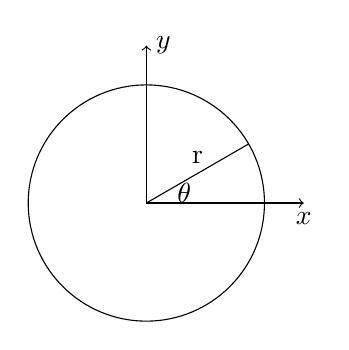
\begin{tikzpicture}
			\def\k{2};
			\node (O) at (0, 0) {};
			\node (A) at (0,1.5) {};
			\node (B) at (30:1.5) {} ;	
			\draw [ ->] (0,0) --  (\k,0)  node[below] {$x$};
			\draw [ ->]  (0,0) -- ( 0,\k)   node[right] {$y$};
			\draw  (0,0) -- (30:1.5) node[midway,above] {r};
			\draw (0,0) circle (1.5cm);
			\path (0,0) ++(15: .5) node{$\theta$};
		\end{tikzpicture}
	\end{center}
\end{frame}	

\begin{frame}
	\alert{ 解:}	这是一个温度场,是非稳恒场,服从传导方程:\\
	$\begin{cases}
		u_t=a^2 [u_{xx}   +u_{yy}] ~~~~ (0< x^2 +y^2 <r_0 ^2, t>0)\\
		u(x,y,t)|_{x^2+y^2=r_0 ^2}= 0 \\
		u(x,y,t)|_{t=0}= \Psi(x,y)
	\end{cases} $\\	
	考虑到圆域边界条件,改用极坐标描述\\
	$\begin{cases}
		\displaystyle	u_t=a^2 [ {	\frac{\partial^2 u }{\partial r^2 } +\frac{1}{r } \frac{\partial u }{\partial r } +
		\frac{1}{r^2 } \frac{\partial ^2 u }{\partial \theta ^2
		} }], ~~~~ (0<r<r_0, t>0)\\
		u(r_0,\theta)=0,~~~~~~~~~~~~ 0<\theta <2\pi 	\\
		u(r,\theta,t )=\Psi(r,\theta) ,~~~~~~~~~~~~ 0<\theta <2\pi 	
	\end{cases} $\\
\end{frame}	

\begin{frame}
	令:$u(r,\theta,t) =R(r)\Theta(\theta)T(t)$,  代回原方程,得:
	\begin{equation*}
		R\Theta T‘=a^2 [ R'' \Theta T + \dfrac{1}{r} R' \Theta T  + \dfrac{1}{r^2} R' \Theta '' T(t)  ]
	\end{equation*}
	整理:
	\begin{equation*}
		-\frac{T'}{a^2T} =\frac{R''}{R}+\frac{1}{r} \frac{R'}{R} +\frac{1}{r^2} \frac{\Theta ''} {\Theta}  =-\lambda
	\end{equation*}
	转化为两个方程:
	\begin{equation*}
		T'(t)+\lambda a^2T(t)=0  ~~~~~....... ~~~~~~(1)
	\end{equation*}
	\begin{equation*}
		r^2 \frac{R'' (r)}{R(r)}+r \frac{R'(r)}{R(r)} + \lambda r^2 +\frac{\Theta ''(\theta)} {\Theta (\theta)} =0  ~~~~~~......~~(2)
	\end{equation*}
\end{frame}	

\begin{frame}
	方程1是衰减模型,已求解!\\
	方程2是固有值问题,可继续分离变量:	
	\begin{equation*}
		r^2 \frac{R'' (r)}{R(r)}+r \frac{R'(r)}{R(r)} + \lambda r^2 =-\frac{\Theta ''(\theta)} {\Theta (\theta)} =\mu  
	\end{equation*}
	得角向固有值问题:
	$ \begin{cases}
		\Theta ''(\theta)+\mu \Theta (\theta) =0 \\
		\Theta (\theta) =	\Theta (\theta+2\pi)  \\
		\Theta' (\theta) =	\Theta' (\theta+2\pi)  
	\end{cases} $\\	
	和径向固有值问题:
	$ \begin{cases}
		r^2 R'' (r)+r R'(r) +( \lambda r^2 -\mu)R(r)=0  \\
		R(r_0)=0
	\end{cases} $\\	
\end{frame}	

\begin{frame}
	角向固有值问题有解,\\
	固有值:
	\begin{equation*}
		\mu=n^2, ~~~~~(n=0,1,2,3...)
	\end{equation*}
	固有函数:
	\begin{equation*}
		\Theta_n(\theta) = a_n \cos(n\theta)+b_n \sin(n\theta), ~~~~~(n=0,1,2,3...)
	\end{equation*}
	\begin{equation*}
		\Theta_n(\theta) = \frac{1}{\sqrt{2\pi}} e^{-i n \theta }, ~~~~~(n=0,1,2,3...)
	\end{equation*}
\end{frame}	

\begin{frame}
	把$\mu=n^2$,代回径向方程,得一类特殊固有值问题:
	$ \begin{cases}
		r^2 R'' (r)+r R'(r) +( \lambda r^2 -n^2)R(r)=0  \\
		R(r_0)=0
	\end{cases} $\\		
\end{frame}	

\begin{frame}
	考虑对圆域的波动方程:\\
	$\begin{cases}
		u_{tt}=a^2 [u_{xx}   +u_{yy}] ~~~~ (0< x^2 +y^2 <r_0 ^2, t>0)\\
		u(x,y,t)|_{x^2+y^2=r_0 ^2}= 0 \\
		u(x,y,t)|_{t=0}= \Psi(x,y) \\
		u_t (x,y,t)|_{t=0}= \varphi  (x,y) 
	\end{cases} $\\		
	如果进行变量分离,也得到特殊固有值问题!
	$\begin{cases}
		r^2 R'' (r)+r R'(r) +( \lambda r^2 -n^2)R(r)=0  \\
		R(r_0)=0
	\end{cases} $\\		
\end{frame}	

\begin{frame}
	处理一下...,令:
	\begin{equation*}
		x=\sqrt{\lambda} r, ~~~~y(x)= R(r) =R(\frac{x}{\sqrt{\lambda}})
	\end{equation*}
	有: 
	\begin{equation*}
		\frac{dy}{dx} = \frac{dR}{dr} \frac{dr}{dx} = \frac{1}{ \sqrt{\lambda}} \frac{dR}{dr}
	\end{equation*}
	\begin{equation*}
		\frac{d^2y}{dx^2} = \frac{1}{\lambda} \frac{dR^2}{dr^2}
	\end{equation*}
\end{frame}	

\begin{frame}
	代回原方程,得:
	\begin{equation*}
		x^2\frac{d^2y}{dx^2} + x\frac{dy}{dx} +(x^2 -n^2)y=0
	\end{equation*}
	称为n(整数)阶贝塞尔方程.\\
	比较与欧拉方程的关系:
	\begin{equation*}
		x^2\frac{d^2y}{dx^2} + x\frac{dy}{dx} +(n^2)y=0
	\end{equation*}
	可以发现贝塞尔方程没有初等函数的表达式解!
\end{frame}	

\begin{frame}
	\frametitle{方程的求解}
	\begin{exampleblock} {例2、求解贝塞尔方程}
		\begin{equation*}
			x^2\frac{d^2y}{dx^2} + x\frac{dy}{dx} +( x^2 -n^2)y=0
		\end{equation*}	
	\end{exampleblock}
	\alert{ 解:}设方程有级数解:
	\begin{equation*}
		y=\sum\limits_{k=0}^{\infty} a_k x^{s+k}
	\end{equation*}	
\end{frame}	

\begin{frame}
	求导:
	\begin{equation*}
		y'=\sum\limits_{k=0}^{\infty} (s+k) a_k x^{s+k-1}
	\end{equation*}	
	\begin{equation*}
		y''=\sum\limits_{k=0}^{\infty} (s+k) (s+k+1) a_k x^{s+k-2}
	\end{equation*}	
	代回原方程,得:
	\begin{equation*}
		\sum\limits_{k=0}^{\infty} [(s+k) ^2 -n^2]  a_k x^{s+k} + \sum\limits_{k=2}^{\infty}  a_{k-2} x^{s+k} =0
	\end{equation*}	
	第一项(k=0)系数应为零:
	\begin{equation*}
		(s+k) ^2 -n^2=0,~~ \to s_1=-n, \qquad s_2=n. 
	\end{equation*}	
\end{frame}	

\begin{frame}
	第二项(k=1)系数应为零:
	\begin{equation*}
		[(s+k) ^2 -n^2] a_1=0,\qquad \to a_1=0. 
	\end{equation*}	
	后面各项(k>1)系数都应为零:
	\begin{equation*}
		[(s+k) ^2 -n^2] a_k+ a_{k-2}=0, ~~~ (k=2,3,4,...)
	\end{equation*}	
	存在递推关系:
	\begin{equation*}
		a_k=-\frac{1}{(s+k) ^2 -n^2 } a_{k-2}
	\end{equation*}	
	由$a_1=0,\qquad \to \qquad a_{2m+1}=0 $。\\
	取$s=n$, 得:
	\begin{equation*}
		a_{2m}=\frac{-1}{(n+2m) ^2 -n^2 } a_{2m-2} =\frac{-1}{2m (2n+2m) } a_{2m-2}, \qquad (m=1,2,3,...)
	\end{equation*}	
\end{frame}	

\begin{frame}
	归纳,得:
	\begin{equation*}
		a_{2m}=(-1)^m  \frac{1}{2^{2m} m! (n+m) (n+m-1)... (n+1) } a_0 
	\end{equation*}	
	取:$a_0=1/2^n n!$, 得:
	\begin{equation*}
		a_{2m}=(-1)^m  \frac{1}{2^{2m+n} m! (n+m) ! }
	\end{equation*}	
	贝塞尔方级数特解:
	\begin{equation*}
		y(x) = \sum\limits_{m=0}^{\infty} a_{2m} x^{n+2m} 
	\end{equation*}	
	分析收敛性,发现:
	\begin{equation*}
		\lim\limits_{m\to \infty}|\frac{ a_{2m+2}} {a_{2m}}|= \lim\limits_{m\to \infty}\frac{ 1}{4(m+1)(n+m+1)} =0
	\end{equation*}	
	说明此级数必为某函数的展开式,称之为贝塞尔函数。
\end{frame}	

\begin{frame}
	\includegraphics[width=0.8\textwidth]{bessel.png}
\end{frame}	

\begin{frame}
	\begin{center}
		\begin{figure}
			\includegraphics[width=4.2cm]{figs/fig1-3-6.png}	
		\end{figure}
	\end{center}
	贝塞尔(Bessel,Friedrich Wilhelm,1784~1846)德国天文学家,数学家,天体测量学的奠基人.
	提出贝塞尔函数,讨论该函数的一系列性质及其求值方法,为解决物理学、天文学和信息学有关问题提供了重要工具。
\end{frame}

\begin{frame}
	\frametitle{作业}
	1、由圆域波动方程导出贝塞尔方程\\
	2、求衰减模型
	\begin{equation*}
		T'(t)+\lambda a^2T(t)=0  ~~~~~....... ~~~~~~(1)
	\end{equation*}
	3、求角向固有值及归一化的固有函数:
	$ \begin{cases}
		\Theta ''(\theta)+\mu \Theta (\theta) =0 \\
		\Theta (\theta) =	\Theta (\theta+2\pi)  \\
		\Theta' (\theta) =	\Theta' (\theta+2\pi)  
	\end{cases} $	
\end{frame}	

\subsection{贝塞尔函数与Gamma函数}

\begin{frame}
	\frametitle{贝塞尔函数}
	零阶贝塞尔函数:
	\begin{equation*}
		J_0(x) = \sum\limits_{m=0}^{\infty} (-1)^m  \frac{1}{m! m! } (\frac{x}{2})^{2m} 
	\end{equation*}	
	n阶贝塞尔函数:
	\begin{equation*}
		J_n(x) = \sum\limits_{m=0}^{\infty} (-1)^m  \frac{1}{m! (n+m) ! } (\frac{x}{2})^{n+2m} 
	\end{equation*}	
	第二类塞尔函数:
	\begin{equation*}
		Y_{\alpha}(x)=\frac{J_{\alpha}(x) \cos (\alpha \pi)-J_{-\alpha}(x)}{\sin (\alpha \pi)}
	\end{equation*}	
	贝塞尔函数在除$x=0$点外的整个实数轴上收敛。
\end{frame}	

\begin{frame}
	\frametitle{$\Gamma$函数及其性质}
	为讨论贝塞尔函数的性质,先定义Gamma函数
	\begin{equation*}
		\Gamma(x)=\int_{0}^{\infty} t^{x-1} e^(-t) dt, \qquad (x>0)
	\end{equation*}	
	\alert{性质1:} Gamma函数有递推式:
	\begin{equation*}
		\Gamma(x+1)=x \Gamma(x)
	\end{equation*}	
	\alert{证明:}  
	\begin{equation*}
	\begin{split}
		\Gamma(x+1)&= \int_{0}^{\infty} t^{x} e^{-t} dt \\
		&= -t^x e^{-t} |_0 ^\infty + x \int_{0}^{\infty} t^{x-1} e^{-t} dt \\
		&= x \int_{0}^{\infty} t^{x-1} e^{-t} dt =x \Gamma(x)
	\end{split}
	\end{equation*}	
\end{frame}	

\begin{frame}
	\alert{性质2:}自变量为正整数的Gamma函数有如下形式:
	\begin{equation*}
		\Gamma(n+1)=n!
	\end{equation*}	
	\alert{证明:}  由递推公式
	\begin{equation*}
	\begin{split}
		\Gamma(x+1)&=x \Gamma(x) \\
		\Gamma(n+1)&=n \Gamma(n) \\
		&=n(n-1)\cdots 1 \Gamma(1) \\
		&=n! \int_{0}^{\infty}  e^{-t} dt \\
		&=n!
	\end{split}
	\end{equation*}	
\end{frame}	

\begin{frame}
	\alert{性质3:} 非正整数点极限为无穷大
	\begin{equation*}
		\lim\limits_{x\to -n }\Gamma(x)=\infty, \qquad (n=0,1,2, \cdots)
	\end{equation*}	
	\alert{证明:}  由递推公式
	\begin{equation*}
	\begin{split}
		\Gamma(x)&=\frac{1}{x} \Gamma(x+1) \\
		\lim\limits_{x\to 0 }	\Gamma(x)&=	\lim\limits_{x\to 0 } \frac{1}{x} \Gamma(x+1) =\infty \\
		\lim\limits_{x\to -1 }	\Gamma(x)&=\lim\limits_{x\to -1 } \frac{1}{x} \Gamma(x+1) =  \lim\limits_{x\to 0 } \frac{1}{x-1} \Gamma(x) =\infty \\
		& \cdots \cdots \\
		\lim\limits_{x\to -n }	\Gamma(x)&=\lim\limits_{x\to -n } \frac{1}{x} \Gamma(x+1) = \lim\limits_{x\to -(n-1) } \frac{1}{x-1} \Gamma(x) =\infty \\
	\end{split}
	\end{equation*}	
\end{frame}	

\begin{frame}
	 推论: 
	\begin{equation*}
		\frac{1}{\Gamma(-n)} =0, \qquad (n=0,1,2, \cdots)
	\end{equation*}	 \vspace{2cm}
	\alert{性质4:} 半正整数$\Gamma$函数 
	\begin{equation*}
		\begin{split}
		\Gamma(\frac{1}{2}) &=\sqrt{\pi} \\ 
		\qquad  \Gamma(m+\frac{1}{2}) &= \frac{(2m-1)!!}{2^m} \sqrt{\pi}
		\end{split}	
	\end{equation*}	
\end{frame}	

\begin{frame}
	现在讨论贝塞尔函数的性质:\\
	\alert{性质1:} 负数阶贝塞尔函数与正数阶贝塞尔函数有如下关系
	\begin{equation*}
		J_{-n}(x)=(-1)^n J_n(x)
	\end{equation*}	
	\alert{证明:}  
	用$\Gamma$ 函数写出贝塞尔函数:
	\begin{equation*}
		J_n(x) = \sum\limits_{m=0}^{\infty} (-1)^m  \frac{1}{m! (n+m) ! } (\frac{x}{2})^{n+2m} 
	\end{equation*}	
	\begin{equation*}
		J_n(x) = \sum\limits_{m=0}^{\infty} (-1)^m  \frac{1}{m! \Gamma(n+m+1) } (\frac{x}{2})^{n+2m} 
	\end{equation*}	
	负数阶塞尔函数可写成
	\begin{equation*}
		J_{(-n)}(x) = \sum\limits_{m=0}^{\infty} (-1)^m  \frac{1}{m! \Gamma(-n+m+1) } (\frac{x}{2})^{-n+2m} 
	\end{equation*}	
\end{frame}	

\begin{frame}
	对于 $m<n$ 的项,由于分母中的Gamma函数为无穷大,所以都为零:
	\begin{equation*}
		J_{(-n)}(x) = \sum\limits_{m=n}^{\infty} (-1)^m  \frac{1}{m! \Gamma(-n+m+1) } (\frac{x}{2})^{-n+2m} 
	\end{equation*}	
	令 $m-n=k$, 有 $m=n+k $, 
	\begin{equation*}
		J_{(-n)}(x) = (-1)^n\sum\limits_{k=0}^{\infty} (-1)^k  \frac{1}{(n+k)! \Gamma(k+1) } (\frac{x}{2})^{n+2k} 
	\end{equation*}	
	\begin{equation*}
		J_{-n} (x) = (-1)^n\sum\limits_{k=0}^{\infty} (-1)^k  \frac{1}{(n+k)! k! } (\frac{x}{2})^{n+2k} =(-1)^n J_{n} (x)
	\end{equation*}	
\end{frame}	

\begin{frame}
	\alert{性质2:} 半整数阶贝塞尔函数与三角函数有如下关系
	\begin{equation*}
		J_{1/2} (x) =\sqrt{\frac{2}{\pi x}} \sin x,  \qquad  J_{-1/2} (x) =\sqrt{\frac{2}{\pi x}} \cos x
	\end{equation*}	
	\alert{证明:}  基于Gamma函数,可以写出半整数阶贝塞尔函数
	\begin{equation*}
		J_n(x) = \sum\limits_{m=0}^{\infty} (-1)^m  \frac{1}{m! \Gamma(n+m+1) } (\frac{x}{2})^{n+2m} 
	\end{equation*}	
	\begin{equation*}
		J_{1/2}(x) = \sum\limits_{m=0}^{\infty} (-1)^m  \frac{1}{m! \Gamma(1/2+m+1) } (\frac{x}{2})^{1/2+2m} 
	\end{equation*}	
\end{frame}	

\begin{frame}
	其中, 
	\begin{equation*}
		\begin{split}
			\Gamma(1/2+m+1) &= (\frac{2m+1}{2}) \Gamma(1/2+m) \\
			& = (\frac{2m+1}{2}\frac{2m-1}{2})  \Gamma(1/2+m-1) \\
			&\cdots \cdots \\
			& = \frac{(2m+1)!!}{2^{m+1}} \Gamma(1/2) \\
			& = \frac{(2m+1)!!}{2^{m+1}} \sqrt{\pi} \\
		\end{split}	
	\end{equation*}	
\end{frame}	

\begin{frame}
	代回,有:
	\begin{equation*}
		J_{1/2}(x) = \sqrt{\frac{2}{\pi x}} \sum\limits_{m=0}^{\infty} (-1)^m  \frac{x^{2m+1}}{(2m+1)!} 
	\end{equation*}	 
	\begin{equation*}
		J_{1/2}(x) = \sqrt{\frac{2}{\pi x}} \sin x  
	\end{equation*}	 
	同理,有  
	\begin{equation*}
		J_{-1/2}(x) = \sqrt{\frac{2}{\pi x}} \cos x  
	\end{equation*}	 
	\alert{证毕!} 
\end{frame}

\begin{frame}
	\frametitle{作业}
	1、证明 $\Gamma(1/2)=\sqrt{\pi}$
	2、证明
	\begin{equation*}
		J_{-1/2}(x) = \sqrt{\frac{2}{\pi x}} \cos x  
	\end{equation*}
\end{frame}

\subsection{贝塞尔函数的性质}

\begin{frame}
	\alert{性质3:} 贝塞尔函数的导数与递推式 \\
	\begin{equation*}
		\begin{split}
			\frac{d}{d x}\left[x^{n} J_{n}(x)\right]= &x^{n} J_{n-1}(x) \\
			\frac{d}{d x}\left[x^{-n} J_{n}(x)\right]=& -x^{-n} J_{n+1}(x) \\
			2 n J_{n}(x)=&xJ_{n-1}(x)+x J_{n+1}(x) \\
			2 J_{n}^{\prime}(x)=&J_{n-1}(x)-J_{n+1}(x)
		\end{split}
	\end{equation*}		
	\alert{证明:}
	\begin{equation*}
		J_n(x) = \sum\limits_{m=0}^{\infty} (-1)^m  \frac{1}{m! \Gamma(n+m+1) } (\frac{x}{2})^{n+2m} 
	\end{equation*}	 
	等于两端乘以$x^n$ 再求导:
	\begin{equation*}
	\begin{split}
		\frac{d}{dx} [x^n J_n(x)]&= \frac{d}{dx}\sum\limits_{m=0}^{\infty} (-1)^m  
		\frac{1}{m! \Gamma(n+m+1) } (\frac{x^{2n+2m}}{2^{n+2m}})\\	
	\end{split}
	\end{equation*}		
\end{frame}	

\begin{frame}
	\begin{equation*}
		\begin{split}
			\frac{d}{dx} [x^n J_n(x)] &=\sum\limits_{m=0}^{\infty} (-1)^m  
			\frac{1}{m! \Gamma(n+m+1) } (\frac{(2n+2m)x^{2n-1+2m}}{2^{n+2m}})\\
			&=x^n\sum\limits_{m=0}^{\infty} (-1)^m  
			\frac{1}{m! \Gamma(n-1+m+1) } (\frac{x^{n-1+2m}}{2^{n-1+2m}})\\ 
			&=x^n J_{n-1}(x)
		\end{split}
	\end{equation*}	
	同理,得:
	\begin{equation*}
		\begin{split}
		\frac{d}{d x}\left[x^{-n} J_{n}(x)\right]&=-x^{-n} J_{n+1}(x) \\
		\end{split}
	\end{equation*}	 
	把上二式左端求导,然后相加相减,得
	\begin{equation*}
		\begin{split}
		2 n J_{n}(x)=&x J_{n-1}(x)+x J_{n+1}(x) \\
		2 J_{n}^{\prime}(x)=&J_{n-1}(x)-J_{n+1}(x)
		\end{split}
	\end{equation*}	 	
\end{frame}

\begin{frame}
	\alert{性质4:} 贝塞尔函数的零点及其正交归一性\\
	\alert{解:}对n(整数)阶贝塞尔方程
	\begin{equation*}
		x^2\frac{d^2y}{dx^2} + x\frac{dy}{dx} +(x^2 -n^2)y=0
	\end{equation*}
	做变量代换 \[ y=\frac{u}{\sqrt{x}}\] 
	得到 u(x)的方程:
	\begin{equation*}
		u'' +[1+\frac{\frac{1}{4}-n^2}{x^2}] u=0
	\end{equation*}
	当$x \to \infty $ 有方程:
	\begin{equation*}
		u'' + u=0 
	\end{equation*}	
\end{frame}	

\begin{frame}
	通解为:\[u=A\cos(x+\theta)\]
	确定A和$\theta$,得n阶贝塞尔函数的渐近公式\\
	\begin{equation*}
		J_{n}(x) \approx \sqrt{\frac{2}{\pi x}} \cos \left(x-\frac{n \pi}{2}-\frac{\pi}{4}\right)
	\end{equation*}
	得零点近似公式:
	\begin{equation*}
		\mu_{m}^{n} \approx m \pi+\frac{n \pi}{2}+\frac{3 \pi}{4}
	\end{equation*}
	对于热传导方程和波动方程,其解为n阶贝塞尔函数$J_n(x)$,对于零边界条件,有$J_n(\sqrt{\lambda}R)=0$,
	基此可确定:\\
	(1)固有值:
	\[ \sqrt{\lambda}R = \mu_{m}^{n}  \qquad \to \qquad \lambda_m ^n =(\frac{\mu_{m}^{n}}{R})^2 \]
\end{frame}	

\begin{frame}
	(2)固有函数:\[F_m ^n(r) = J_n (\frac{\mu_{m}^{n}}{R}r) \]
	固有函数体现塞尔函数的正交归一性:
	\begin{equation*}
		\int_0 ^R r J_n (\frac{\mu_{m}^{n}}{R}r) J_n (\frac{\mu_{k}^{n}}{R}r) dr =?
	\end{equation*}
	\alert{证明:}对径向方程做等价变换
	\begin{equation*}
		r^2 F''+r F' +(\lambda r^2 -n^2)F=0 
	\end{equation*}	
	\begin{equation*}
		r F''+ F' +((\frac{\mu_{m}^{n}}{R})^2 r -\frac{n^2}{r})F=0  
	\end{equation*}	
	\begin{equation*}
		(r F')' +((\frac{\mu_{m}^{n}}{R})^2 r -\frac{n^2}{r})F=0  
	\end{equation*}	
\end{frame}	

\begin{frame}
	令:\[J_n (\frac{\mu_{m}^{n}}{R}r)=F_1, \qquad J_n (\frac{\mu_{k}^{n}}{R}r) =F_2\]
	有
	\begin{equation*}
		(r F_1')' +((\frac{\mu_{m}^{n}}{R})^2 r -\frac{n^2}{r})F_1=0  \cdots (1)
	\end{equation*}	 
	\begin{equation*}
		(r F_2')' +((\frac{\mu_{m}^{n}}{R})^2 r -\frac{n^2}{r})F_2=0  \cdots (2) 
	\end{equation*}	
	$(1)\times F_2,  (2)\times F_1,$所得两次相减,并做积分,有
	\begin{equation*}	
		\int_0 ^R \left[\left(\frac{\mu_{m}^{(n)}}{R}\right)^{2}-\left(\frac{\mu_{k}^{(n)}}{R}\right)^{2}\right] r F_{1} F_{2} dr 
		=\int_0 ^R  [F_{1}\left(r F_{2}^{\prime}\right)^{\prime}-F_{2}\left(r F_{1}^{\prime}\right)^{\prime}] dr
	\end{equation*}
\end{frame}	

\begin{frame}
	\begin{equation*}
		\begin{split}
			=& [rF_1F_2']|_0 ^R - [rF_2F_1']|_0 ^R + \int_0 ^R rF_2'F_1 dr - \int_0 ^R rF_1'F_2 dr\\
			=& \int_0 ^R rF_2'F_1 dr - \int_0 ^R rF_1'F_2 dr\\
			=& 0
		\end{split}
	\end{equation*}	
	\begin{equation*}	
		\to \qquad	\int_0 ^R r F_{1} F_{2} dr = 0
	\end{equation*}
	正交性,\alert{证毕!}
\end{frame}	

\begin{frame}
	下面证明归一性:
	\begin{equation*}
		r^2 F''+r F' +(\lambda r^2 -n^2)F=0 
	\end{equation*}	
	\begin{equation*}
		2r^2 F'F''+2r (F')^2 +(\lambda r^2 -n^2)F'F=0 
	\end{equation*}	
	 整理:
	\begin{equation*}
		[r^2 (F')^2 + (\lambda r^2 -n^2)F^2]'=2 \lambda rF^2
	\end{equation*}	
\end{frame}	

\begin{frame}
	\begin{equation*}
		\begin{split}
			\int_0 ^R r F~^2 dr =& \frac{1}{2\lambda} \int_0 ^R [r^2 (F')^2 + (\lambda r^2 -n^2)F^2]' dr  \\
			=& \frac{1}{2\lambda} |[r^2 (F')^2 + (\lambda r^2 -n^2)F^2 |_0 ^R \\
			=& \frac{1}{2\lambda} R^2 (F'(R))^2 \\
			=& \frac{1}{2} R^2 [J'_n(\mu_m ^n)]^2 \\
			=& \frac{R^2}{2} [J_{n+1}(\mu_m ^n)]^2
		\end{split}
	\end{equation*}	
\end{frame}	

\begin{frame}
	\frametitle{应用实例}
	求解圆域热传导问题 \\
	$\left\{
		\begin{array}{l}
		\dfrac{\partial u}{\partial t}=a^{2}\left(\dfrac{\partial^{2} u}{\partial r^{2}}+\dfrac{1}{r} 
		\dfrac{\partial u}{\partial r}+\dfrac{1}{r^{2}} \dfrac{\partial^{2} u}{\partial \theta^{2}}\right), 0<r<R, 0<\theta<2 \pi \\
		\left. u\right|_{r=R}=0,\left.u\right|_{t=0}=\varphi(r, \theta)
	\end{array}
	\right. $\\
	\alert{解:} 令 
	\begin{equation*}
		u(r,\theta,t)= T(t) V(r, \theta) 
	\end{equation*}	
	代入方程,进行第一次分离变量,得衰减方程:\[T'+\lambda a^2 T=0, \qquad \cdots (1) \]	
\end{frame}

\begin{frame}
	及亥姆霍兹方程:
	$\left\{
	\begin{array}{l}
		\frac{\partial^{2} V}{\partial r^{2}}+\frac{1}{r} \frac{\partial V}{\partial r}+\frac{1}{r^{2}} 
		\frac{\partial^{2} V}{\partial \theta^{2}}+\lambda V=0, 0<r<R, 
		0 \leq \theta \leq 2 \pi \\
		\left.V\right|_{r=R}=0, 0 \leq \theta \leq 2 \pi
		\end{array}
	\right.$\\
	令\[V(r, \theta) =F(r)G(\theta)\], 代入亥姆霍兹方程, 得两个方程\\
	\[G''+\mu G=0, \qquad \cdots (2) \]
	\[r^2 F''+r F' +(\lambda r^2 -\mu )F=0, \qquad \cdots (3) \]
\end{frame}	

\begin{frame}
	方程(1)的解为:\[T(t)=Ae^{-\lambda a^2 t}\]
	方程(2)的解为:\[G(\theta)=C_1\cos\sqrt{\mu}\theta + C_2\sin \sqrt{\mu}\theta \]
	由周期性边界条件,有$G(2\pi)=G(0)$, 必有$\cos \sqrt{\mu}\theta =1 $, 得\\
	固有值:
	\[\mu = n^2, \qquad (n=0,1,2,\cdots)\]
	固有函数:
	\[G_0(\theta)=\frac{1}{2}a_0, G_n(\theta)= a_n\cos n \theta + b_n \sin n \theta, \qquad (n=0,1,2,\cdots)\]
	固有函数也可写成 $ G_n(theta)=a_n e^{-i n \theta} =\frac{1}{\sqrt{2\pi}} e^{-i n \theta}$
\end{frame}	

\begin{frame}
	将固有值代入方程(3),得方程 
	\[r^2 F''+r F' +(\lambda r^2 -n^2 )F=0 \]
	令 $x=\sqrt{\lambda} r, y(x)=F(x/\sqrt{\lambda})$, 
	方程转化为标准整数贝赛尔方程:
	\begin{equation*}
		x^2\frac{d^2y}{dx^2} + x\frac{dy}{dx} +(x^2 -n^2)y=0
	\end{equation*}
	则方程(3)的解用贝赛尔函数的零点表示:\\
	固有值:
	\[\lambda_m ^n =(\frac{\mu_{m}^{n}}{R})^2 \]
	固有函数:\[F_m ^n(r) = J_n (\frac{\mu_{m}^{n}}{R}r) \]
\end{frame}	
\begin{frame}
	原方程的基本解为:
	\begin{equation*}
		u(r,\theta,t) =F_m ^n (r) G_n(\theta) e^{-\lambda_m a^2 t}
	\end{equation*}
	叠加解为:
	\begin{equation*}
		u(r,\theta,t) =\sum_{n=0}^{\infty} \sum_{m=0}^{\infty} A_m ^n F_m ^n (r) G_n(\theta) e^{-\lambda_m a^2 t}
	\end{equation*}
	应用初值条件, 
	\begin{equation*}
		\varphi(r, \theta)=\sum_{n=0}^{\infty} \sum_{m=0}^{\infty} A_m ^n F_m ^n (r) G_n(\theta) 
	\end{equation*}
	利用正交归一性确定系数$A_m ^n$
\end{frame}	

\begin{frame}
	\begin{equation*}
		 \int_0 ^{2\pi} G_k ^* (\theta) \varphi(r, \theta) d\theta =\sum_{n=0}^{\infty} \sum_{m=0}^{\infty} A_m ^n F_m ^n (r) \int_0 ^{2\pi} G_n(\theta) G_k(\theta) d\theta
	\end{equation*}
	\begin{equation*}
		 \int_0 ^{2\pi} G_n  ^* (\theta) \varphi(r, \theta) d\theta = \sum_{m=0}^{\infty} A_m ^n F_m ^n (r)
	\end{equation*}
	{\small \begin{equation*}
		\int_0 ^{R} \int_0 ^{2\pi} G_n ^* (\theta) r J_n (\frac{\mu_{k}^{n}}{R}r) \varphi(r, \theta) d\theta dr = \sum_{m=0}^{\infty} A_m ^n \int_0 ^{R} r J_n (\frac{\mu_{k}^{n}}{R}r)J_n (\frac{\mu_{m}^{n}}{R}r) dr
	\end{equation*}}
	\begin{equation*}
		\int_0 ^{R} \int_0 ^{2\pi} G_n ^* (\theta) r J_n (\frac{\mu_{m}^{n}}{R}r) \varphi(r, \theta) d\theta dr = A_m ^n \frac{R^2}{2} [J_{n+1}(\mu_m ^n)]^2
	\end{equation*}
\end{frame}	

\begin{frame}
	\begin{equation*}
		\to A_m ^n=	\frac{2}{R^2[J_{n+1}(\mu_m ^n)]^2} \int_0 ^{R} \int_0 ^{2\pi} G_n ^* (\theta) r J_n (\frac{\mu_{m}^{n}}{R}r) \varphi(r, \theta) d\theta dr 
	\end{equation*}
\end{frame}

\begin{frame}
	\frametitle{作业}
	1、证明 
	\begin{equation*}
		J_{3/2}(x)=\sqrt{\frac{2}{\pi x}} [\frac{1}{x}\sin x -\cos x]
	\end{equation*}
	2、证明
	\begin{equation*}
		\frac{d}{d x}\left[x^{-n} J_{n}(x)\right]=-x^{-n} J_{n+1}(x) 
	\end{equation*}	
	3、用分离变量法分析球域热传导方程
	\begin{equation*}
		u_t=a^2 (u_{xx}+u_{yy}+u_{zz}), \qquad (0<r<R)
	\end{equation*}	
\end{frame}	
%%%%%%%%%%%%%%%%%%%%%%%%%%%%%%%%%%%%%%%%%%%%%%%%